\documentclass[12pt,a4paper,oneside]{report}
\usepackage[a4paper,margin=1in]{geometry}
\usepackage[T1]{fontenc}
\usepackage[utf8]{inputenc}
\usepackage{lmodern,microtype}
\usepackage{setspace,graphicx,booktabs,tabularx,array,enumitem,hyperref,xcolor,tikz,float,url}
\usetikzlibrary{arrows.meta,positioning}
\hypersetup{colorlinks=true,linkcolor=black,citecolor=blue!50!black,urlcolor=blue!50!black}
\setstretch{1.18}
\renewcommand{\arraystretch}{1.15}
\begin{document}
\begin{titlepage}\centering
\vspace*{0.7cm}
{\Large\bfseries UCS503P -- Project Report\par}
\vspace{1.5cm}
{\Huge\bfseries ResearchAgent: An Autonomous AI Agent for Stock and Company Research\par}
\vspace{0.5cm}{\Large Prototype-Stage Report\par}
\vspace{1.5cm}
{\large\bfseries Submitted by\par}\vspace{0.4cm}
Ananya Khanduja, CSED \quad 1024030693\\
Garv Sharma, CSED \quad 1024030695\\
Vishwa Choudhary, CSED \quad 1024030668\\
\vspace{1.2cm}
{\large\bfseries Submitted to\par}\vspace{0.3cm}
{\Large Paramveer Ma'am\par}
\vfill
{\large Mid-Semester Evaluation\par}
{\large Computer Science and Engineering Department\par}
{\large Thapar Institute of Engineering and Technology, Patiala\par}
\vspace{0.5cm}{\large October 2026\par}
\end{titlepage}

\pagenumbering{roman}
\chapter*{Abstract}
Researching a listed company commonly requires users to move between financial-data portals, news sources, and search engines before assembling a coherent view. This fragmentation increases effort and makes the resulting notes inconsistent. ResearchAgent is a course project that proposes a web-based, tool-using AI agent to accept a company name or ticker, gather available evidence through external tools, and synthesise it into a structured research brief.

The target architecture separates a React, Vite, and TypeScript frontend from a stateless Go HTTP API. Its proposed agent loop follows a Plan--Act--Observe--Reflect--Synthesise pattern and uses search, financial-data, and news tools with layered fallbacks. The proposal prioritises free-tier services and defines median time-to-report (TTR) of at most 60 seconds for a resolved NSE/BSE ticker as its primary performance target.

At the prototype stage, the frontend includes a landing page and initial routing, along with agent-activity and tool-indicator components and shared TypeScript types. These provide part of the user-interface foundation. Complete end-to-end execution, report completeness, source grounding, and performance have not been established by the frontend artifacts alone and require integration testing. This report documents the problem, design, current implementation evidence, evaluation plan, limitations, and next steps without presenting unmeasured targets as achieved results.

\noindent\textbf{Keywords:} AI agent, company research, tool orchestration, financial information, Go, React, TypeScript.

\tableofcontents
\listoffigures
\listoftables
\clearpage
\pagenumbering{arabic}

\chapter{Introduction}
\section{Background and Context}
Preliminary research on a listed company may involve reviewing financial snapshots, recent news, company and sector context, competitors, and potential risk factors. These materials are distributed across different websites and vary in freshness and format. A user must identify relevant sources, cross-check claims, and organise the information into a consistent brief.

Large language models can assist with synthesis, but a model-only answer may be incomplete or unsupported if it is not grounded in retrieved evidence. A tool-using agent offers a more structured approach: plan research steps, call external tools, inspect their outputs, retry when evidence is insufficient, and generate a report from the gathered context. The engineering challenge is to coordinate tools reliably and communicate uncertainty when data is unavailable.

ResearchAgent targets this problem with a lightweight web application intended for students and individual investors. The immediate engineering objective is a measurable research workflow for one company at a time, rather than novel model research or stock-price prediction.

\subsection{Problem Statement}
The project proposal identifies four pain points:
\begin{itemize}[leftmargin=*]
\item \textbf{Fragmentation:} financial information, news, and qualitative context live on separate sites and require manual cross-referencing.
\item \textbf{Cost barriers:} paid data providers and model APIs may be inaccessible to students and retail investors.
\item \textbf{Inconsistent structure:} manually compiled notes vary in coverage and organisation.
\item \textbf{Freshness and completeness:} manual snapshots can become stale and omit relevant news or risks.
\end{itemize}
ResearchAgent aims to reduce this effort by gathering available evidence and organising it into a repeatable brief. It is an informational research aid, not a substitute for professional financial advice.

\section{Project Objectives}
\begin{enumerate}[leftmargin=*]
\item Provide a web interface that accepts a company name or stock ticker.
\item Design an agent loop that plans research and dispatches search, financial-data, and news tools.
\item Synthesize retrieved context into six sections: overview, financial snapshot, news, competitive landscape, risk factors, and bull/bear investment summary.
\item Improve resilience through layered fallbacks and graceful handling of empty or unavailable results.
\item Evaluate TTR, ticker-resolution accuracy, report completeness, fallback frequency, and endpoint availability.
\item Keep deployment practical through a decoupled React frontend and Go API, targeting free-tier hosting and no required managed database.
\end{enumerate}

\section{Prototype Scope}
The repository work documented for this report includes a frontend landing page, initial routing, reusable agent-activity and tool-indicator components, and shared TypeScript types. The proposal describes a broader target system including backend orchestration, data tools, fallbacks, and report generation. Chapter~\ref{chap:results} distinguishes these frontend artifacts from capabilities that still need end-to-end verification.

\chapter{Methodology and Design}
\section{System Architecture}
The target system separates user interaction from research orchestration. The frontend collects a company or ticker and presents activity and the eventual report. The Go API coordinates the request, invokes the model and data tools, and returns structured output. External sources provide search results, financial data, and news.

\subsection{High-Level Design}
Figure~\ref{fig:architecture} shows the intended architecture. It is a design view, not proof that every component is integrated and tested.
\begin{figure}[H]\centering
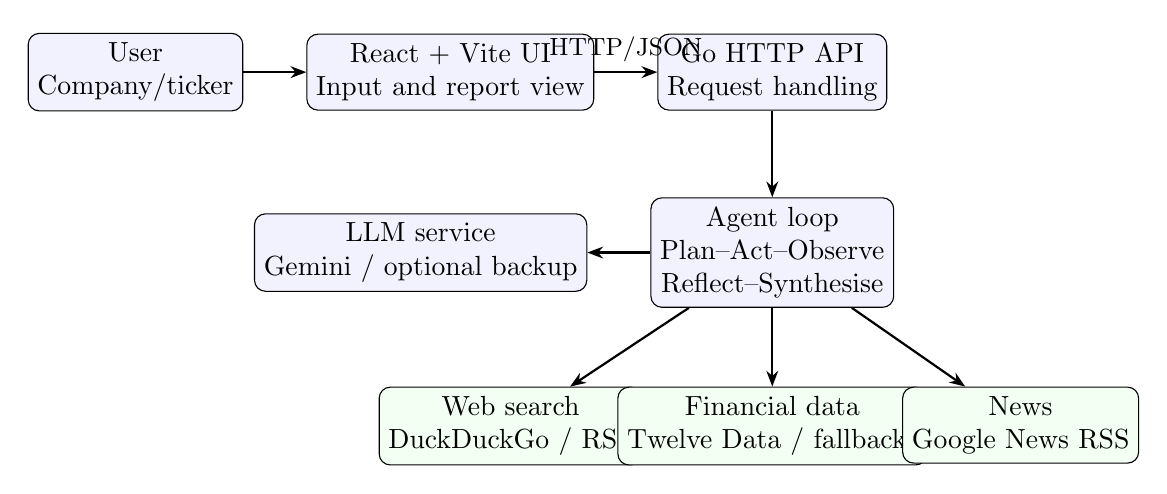
\begin{tikzpicture}[node distance=0.7cm and 0.8cm,box/.style={draw,rounded corners,align=center,minimum width=2.6cm,minimum height=0.8cm,fill=blue!5},tool/.style={draw,rounded corners,align=center,minimum width=2.5cm,minimum height=0.75cm,fill=green!5},arr/.style={-{Stealth[length=2mm]},thick}]
\node[box] (user) {User\\Company/ticker};
\node[box,right=of user] (ui) {React + Vite UI\\Input and report view};
\node[box,right=of ui] (api) {Go HTTP API\\Request handling};
\node[box,below=1.1cm of api] (agent) {Agent loop\\Plan--Act--Observe\\Reflect--Synthesise};
\node[tool,below left=1cm and 0.1cm of agent] (search) {Web search\\DuckDuckGo / RSS};
\node[tool,below=1cm of agent] (finance) {Financial data\\Twelve Data / fallbacks};
\node[tool,below right=1cm and 0.1cm of agent] (news) {News\\Google News RSS};
\node[box,left=of agent] (llm) {LLM service\\Gemini / optional backup};
\draw[arr] (user)--(ui);\draw[arr] (ui)--node[above,font=\small]{HTTP/JSON}(api);
\draw[arr] (api)--(agent);\draw[arr] (agent)--(llm);
\draw[arr] (agent)--(search);\draw[arr] (agent)--(finance);\draw[arr] (agent)--(news);
\end{tikzpicture}
\caption{Proposed ResearchAgent architecture. Integration and runtime behaviour require validation.}
\label{fig:architecture}
\end{figure}

The intended request flow is: (1) accept a company or ticker; (2) resolve or validate the ticker; (3) plan research steps; (4) dispatch tools and inspect their results; (5) retry or use fallbacks when evidence is insufficient; and (6) synthesise a structured report for display. The implementation should retain source provenance and avoid claiming completeness when sources fail.

\subsection{Agent Orchestration}
The proposal specifies a Plan--Act--Observe--Reflect--Synthesise loop. Planning identifies the information needed. Acting dispatches search, financial-data, or news calls. Observation records tool output. Reflection checks whether the evidence is sufficient and whether a retry or fallback is warranted. Synthesis organises the retrieved context into the final brief. Explicit tool boundaries allow source failures to be handled without treating missing data as facts.

\subsection{Technical Stack}
\begin{table}[H]\centering\small
\begin{tabularx}{\textwidth}{>{\raggedright\arraybackslash}p{3.3cm}X}
\toprule \textbf{Technology} & \textbf{Intended role}\\\midrule
Go standard library & HTTP API and backend orchestration.\\
React, TypeScript, Vite & Web interface, typed components, and frontend build.\\
Tailwind CSS & Responsive, dark-mode-first styling.\\
Gemini API & Primary language-model service for planning and synthesis.\\
OpenRouter & Optional model-access fallback, subject to configuration.\\
Twelve Data & Optional primary financial-data API.\\
Yahoo Finance and Screener.in & Layered fallback sources; availability is not guaranteed.\\
DuckDuckGo HTML search and Google News RSS & Search and news retrieval with fallback behaviour.\\
Render & Intended hosting for API and static frontend.\\
Git/GitHub & Version control and collaboration.\\
\bottomrule
\end{tabularx}
\caption{Proposed technology stack and responsibilities.}
\label{tab:stack}
\end{table}

\section{Implementation Details}
\subsection{Frontend Input and Navigation}
The frontend is located in \texttt{code/analyst-agent-web}. The prototype increment includes a dedicated home page at \texttt{src/pages/Home.tsx}, initial application routing in \texttt{src/App.tsx}, and styling and configuration updates. These establish the entry point for a company/ticker query and the initial navigation structure. A route in the frontend does not itself prove that a report page or complete API round trip is operational.

\subsection{Agent Activity UI and Shared Types}
The frontend increment adds \texttt{src/components/AgentThinking.tsx} and \texttt{src/components/ToolCallBadge.tsx}, and extends \texttt{src/types/index.ts}. These components are intended to represent agent progress and tool activity, while shared types provide consistent structures for agent steps, tool calls, messages, and report data. Their presence establishes presentation primitives; live event streaming and backend integration must be tested separately.

\subsection{Backend and Data-Source Design}
The proposal defines a Go HTTP API with an agent route and dedicated search, financial-data, and news tools. Twelve Data is the optional primary financial source, with Yahoo Finance and Screener.in described as fallback sources. Search is intended to try DuckDuckGo and use a Google News RSS fallback when appropriate; Google News RSS also supplies dedicated news retrieval. Public and unofficial sources may change, throttle requests, or become unavailable. Timeouts, bounded retries, and clear error handling are therefore important. The degree of implementation of each backend module should be confirmed against source code and passing tests before being claimed as complete.

\subsection{Report Synthesis}
The intended six sections are: (1) company overview, (2) financial snapshot, (3) recent news, (4) competitive landscape, (5) risk factors, and (6) bull/bear investment summary. Synthesis should be grounded in retrieved tool output. Missing information should be explicitly marked rather than filled with invented values, and the brief should be labelled informational, not financial advice.

\section{Resilience and Deployment}
Risks include source instability, rate limits, model/API quotas, incorrect ticker resolution, and unsupported generated claims. The proposal's mitigations include layered fallbacks, graceful degradation, retries when evidence is insufficient, and source-grounded synthesis. The intended deployment separates the stateless Go API from the static frontend, enabling independent build and deployment. CI is planned to build and vet Go code and type-check/build the frontend; pipeline status should only be reported after verification.

\chapter{Results and Evaluation}
\label{chap:results}
\section{Prototype Status}
Table~\ref{tab:status} separates documented frontend work from end-to-end capabilities that require further verification.
\begin{table}[H]\centering\small
\begin{tabularx}{\textwidth}{>{\raggedright\arraybackslash}p{3.2cm}X>{\raggedright\arraybackslash}p{2.5cm}}
\toprule \textbf{Capability} & \textbf{Evidence / acceptance check} & \textbf{Status}\\\midrule
Landing page & Home page source under \texttt{src/pages/Home.tsx}. & Frontend implemented\\
Initial routing & Route setup in \texttt{src/App.tsx}. & Frontend implemented\\
Agent activity UI & \texttt{AgentThinking.tsx}. & Component added; live integration unverified\\
Tool indicator & \texttt{ToolCallBadge.tsx}. & Component added\\
Shared agent/report types & \texttt{src/types/index.ts}. & Types added\\
Ticker resolution & Test known company names and NSE/BSE symbols. & Requires test evidence\\
End-to-end execution & Verify tool calls, synthesis, and returned report. & Requires integration validation\\
Six-section completeness & Review each section against retrieved sources. & Not measured here\\
Median TTR & Measure request receipt to synthesis completion. & Not measured here\\
Endpoint availability & Probe endpoint during a documented window. & Not measured here\\
\bottomrule
\end{tabularx}
\caption{Prototype status and outstanding verification.}
\label{tab:status}
\end{table}

\section{Testing Methodology}
The following tests are proposed for the next validation pass; results should be recorded only after execution.
\subsection{Frontend tests}
\begin{itemize}[leftmargin=*]
\item Confirm the landing page renders without console errors.
\item Test empty input, whitespace, a known ticker, and a company-name query.
\item Confirm navigation and validation behaviour for valid and invalid inputs.
\item Test agent-activity and tool-indicator components with sample data, including empty steps and failed tool results.
\end{itemize}
\subsection{Backend and integration tests}
\begin{itemize}[leftmargin=*]
\item Verify health and API routes, status codes, and JSON response structure.
\item Exercise each tool with valid queries and simulated timeout, rate-limit, and empty-result conditions.
\item Verify a complete request through planning, tool dispatch, observation, retry where applicable, synthesis, and rendering.
\item Confirm source failures appear as missing evidence rather than fabricated financial facts.
\end{itemize}
\subsection{Data-grounding review}
For a sample of generated reports, compare financial figures and news claims with the sources returned during the run. Record whether each claim is supported and whether missing data or uncertainty is communicated. A report should not pass solely because all six headings are present.

\section{Performance Metrics}
The proposal defines time-to-report (TTR) as the primary metric, with a target median of at most 60 seconds for a resolved NSE/BSE ticker. Secondary metrics are ticker-resolution accuracy, data completeness, fallback trigger rate, and endpoint availability. These are targets and evaluation criteria, not measured achievements.
\begin{table}[H]\centering\small
\begin{tabularx}{\textwidth}{>{\raggedright\arraybackslash}p{3cm}X>{\raggedright\arraybackslash}p{3cm}}
\toprule \textbf{Metric} & \textbf{Measurement} & \textbf{Current evidence}\\\midrule
Time-to-report & Median time from API receipt to synthesis over resolved tickers. & Target $\leq 60$ s; not measured\\
Ticker-resolution accuracy & Correct mappings divided by tested company-name inputs. & Baseline required\\
Data completeness & Reports with six non-empty, source-grounded sections divided by attempts. & Not measured\\
Fallback trigger rate & Runs invoking fallback divided by total runs, by source. & Not measured\\
Availability & Successful endpoint probes divided by total probes over a stated window. & Not measured\\
\bottomrule
\end{tabularx}
\caption{Evaluation metrics and evidence status.}
\label{tab:metrics}
\end{table}
The proposal recommends a pilot of 20--30 companies spanning large-cap, mid-cap, and small-cap NSE/BSE listings. A test log should record input, resolved ticker, timestamps, tool and fallback events, section completeness, and manual source-grounding results. Median latency should be reported with sample size and failures; a single successful run cannot establish the target.

\section{Analysis}
The frontend work establishes an entry point and reusable presentation components. These are necessary building blocks but do not establish that the complete pipeline meets performance or quality targets. The next milestone is a reproducible end-to-end request demonstrating ticker handling, tool invocation, source-grounded synthesis, and report rendering. Source fallback may improve resilience while increasing latency, so this trade-off should be measured. Report quality must be evaluated separately from response speed.

\chapter{Conclusion}
\section{Summary of Work}
ResearchAgent aims to reduce manual effort in preliminary company research by coordinating public information retrieval and model synthesis into a structured investment brief. Its proposed architecture combines a React/TypeScript frontend, Go API, tool-using agent loop, and layered search, financial-data, and news sources. The documented frontend prototype includes a landing page, initial routing, agent-activity and tool-indicator components, and shared types. End-to-end correctness, report completeness, source grounding, and TTR remain to be established through testing.

\section{Key Findings}
\begin{itemize}[leftmargin=*]
\item Separating frontend interaction from backend orchestration provides a clear system boundary.
\item Agent-activity components and shared types establish a foundation for representing tool use in the interface.
\item Source fallbacks and explicit handling of missing evidence are central when relying on public data and free-tier services.
\item Credible evaluation requires both operational metrics and factual-grounding review; speed alone is insufficient.
\end{itemize}

\section{Future Work and Recommendations}
\begin{enumerate}[leftmargin=*]
\item Complete and verify the end-to-end API path from ticker input to rendered report.
\item Implement or validate ticker resolution and all three research tools, including fallbacks.
\item Connect live agent-step events to the frontend and test success, retry, empty, and error states.
\item Generate the six-section brief with source references and explicit missing-data handling.
\item Add route-level tests, Go build/vet checks, frontend type checking, and repeatable CI.
\item Run the proposed 20--30-company pilot and report actual TTR, resolution accuracy, completeness, fallback rate, and availability.
\item Add bounded retries, timeouts, request pacing, and caching where appropriate.
\item Review privacy, source terms, and deployment configuration; keep API keys out of source control.
\end{enumerate}

\section{Final Remarks}
ResearchAgent applies established engineering practices to an information-access problem: modular architecture, explicit tool orchestration, source fallback, typed interfaces, and measurable evaluation. Its value depends on the quality and traceability of retrieved evidence, not merely on fluent output. The next stage should prioritise a working end-to-end slice and transparent evaluation against the project's stated criteria.

\begin{thebibliography}{99}
\bibitem{proposal} A. Khanduja, G. Sharma, and V. Choudhary, \textit{ResearchAgent: An Autonomous AI Agent for Stock and Company Research}, Project Proposal for UCS503P, Thapar Institute of Engineering and Technology, August 25, 2026.
\bibitem{react} Meta Open Source, \textit{React Documentation}. Available: \url{https://react.dev/}. Accessed October 2026.
\bibitem{vite} Vite Contributors, \textit{Vite Documentation}. Available: \url{https://vite.dev/}. Accessed October 2026.
\bibitem{ts} Microsoft, \textit{TypeScript Documentation}. Available: \url{https://www.typescriptlang.org/docs/}. Accessed October 2026.
\bibitem{go} The Go Authors, \textit{Go Documentation}. Available: \url{https://go.dev/doc/}. Accessed October 2026.
\bibitem{gemini} Google, \textit{Gemini API Documentation}. Available: \url{https://ai.google.dev/gemini-api/docs}. Accessed October 2026.
\bibitem{twelvedata} Twelve Data, \textit{API Documentation}. Available: \url{https://twelvedata.com/docs}. Accessed October 2026.
\bibitem{render} Render, \textit{Documentation}. Available: \url{https://render.com/docs}. Accessed October 2026.
\end{thebibliography}
\end{document}
